\documentclass[a4paper,10pt]{article}

\usepackage[english]{babel}
\usepackage{graphicx}
\usepackage[colorlinks, linkcolor=black, citecolor=black, urlcolor=black]{hyperref}
\usepackage{geometry}
\geometry{tmargin=3cm, bmargin=2.2cm, lmargin=2.2cm, rmargin=2cm}
\usepackage{todonotes} %Used for the figure placeholders
\usepackage{ifthen}
\usepackage{pgfplots}
\pgfplotsset{compat=1.18}
\usepackage{pgfplots}
\usepackage{listings}
\usepackage{float}
\usepackage{xcolor} % good practice to load this explicitly before using \color
\usepackage{url} % of \usepackage{hyperref}

% Your name and student number must be filled in on the title page found in
% titlepage.tex.
\lstdefinelanguage{CUDA}{
  language=C++,
  morekeywords={
    __global__, __device__, __host__, __shared__, __constant__,
    __syncthreads, __threadfence_block, __threadfence, __threadfence_system,
    threadIdx, blockIdx, blockDim, gridDim
  },
  sensitive=true
}

% Algemene stijl
\lstset{
  language=CUDA,            % Use custom defined language
    basicstyle=\ttfamily\footnotesize,      % Monospaced font, small
    keywordstyle=[1]\color{blue}\bfseries,  % Mnemonics in blue and bold
    keywordstyle=[2]\color{purple},         % Registers in purple
    keywordstyle=[3]\color{brown}\bfseries, % Labels in brown and bold
    keywordstyle=[4]\color{teal}\bfseries,  % Constants and preprocessor in teal
    commentstyle=\color{gray},              % Comments in gray
    stringstyle=\color{red},                % Strings in red
    numbers=left,                           % Line numbers on the left
    numberstyle=\tiny\color{gray},          % Line number style
    stepnumber=1,                           % Line numbering step
    numbersep=5pt,                          % Space between line numbers and code
    breaklines=true,                        % Line breaking
    backgroundcolor=\color{gray!20},        % Light gray background
    frame=single,                           % Single frame around the code block
    captionpos=b,                           % Caption position at the bottom
    escapeinside={\%*}{*)},                 % Escape to LaTeX with %*...*)
}

\begin{document}
\newboolean{anonymize}
% Uncomment to create an anonymized version of your report
%\setboolean{anonymize}{true}

\begin{titlepage}
    \newpage
    \thispagestyle{empty}
    \frenchspacing
    \hspace{-0.2cm}
    \includegraphics[height=3.4cm]{sedes}
    \hspace{0.2cm}
    \rule{0.5pt}{3.4cm}
    \hspace{0.2cm}
    \begin{minipage}[b]{8cm}
        \Large{Katholieke\newline Universiteit\newline Leuven}\smallskip\newline
        \large{}\smallskip\newline
        \textbf{Department of\newline Computer Science}\smallskip
    \end{minipage}
    \hspace{\stretch{1}}
    \vspace*{3.2cm}\vfill
    \begin{center}
        \begin{minipage}[t]{\textwidth}
            \begin{center}
                \LARGE{\rm{\textbf{\uppercase{Advanced computer architecture}}}}\\
                \Large{\rm{project}}
            \end{center}
        \end{minipage}
    \end{center}
    \vfill
    \hfill\makebox[8.5cm][l]{%
        \vbox to 7cm{\vfill\noindent
            \ifthenelse{\boolean{anonymize}}{%
                {\rm \textbf{Anonymized}}\\
                {\rm Academic year 2025--2026}
            }{%
                {\rm \textbf{Thibaut Beck}}\\
                {\rm \textbf{Wannes Paesschesoone}}\\
              [2mm]
                {\rm Academic year 2025--2026}
            }
        }
    }
\end{titlepage}


\tableofcontents
\newpage
\section{Introduction}
This report talks about the implementation of a point cloud to voxel grid filter.
\section{Theory}

\subsection{Point Cloud}
A \textbf{point cloud} is a collection of data points defined in a three-dimensional coordinate system.  
Each point represents a position in space, typically described by $(x, y, z)$ coordinates.  
Point clouds are commonly acquired using 3D scanners, LiDAR sensors, or photogrammetry systems.  
They are used in applications such as 3D modeling, robotics, mapping, and computer vision.

\subsection{Voxel}
A \textbf{voxel} (volumetric pixel) is the smallest unit of a 3D grid, similar to how a pixel is the smallest unit of a 2D image.  
Voxels divide 3D space into uniform cubes, allowing volumetric representations of shapes or environments.  
They are used in 3D reconstruction, simulation, gaming, and medical imaging.

\subsection{Pointcloud to Voxel Grid Filtering}
\textbf{Pointcloud to voxel grid filtering} converts an unstructured point cloud into a regular 3D grid.  
Space is divided into equal-sized voxels, and each point is assigned to its corresponding voxel.  
This reduces data density, removes redundant points, and creates a structured representation that is easier and faster to process for tasks such as downsampling and spatial queries.

\subsection{Morton Codes}
\textbf{Morton codes} (also called Z-order curves) are a method of encoding multi-dimensional coordinates into a single integer value.  
They work by bit-interleaving the binary coordinates (e.g., $x$, $y$, $z$).  
This encoding preserves spatial locality, making it useful for data structures such as octrees and for accelerating spatial queries on GPUs.

\subsection{CUDA Thrust Library}
The \textbf{CUDA Thrust library} is a parallel algorithms library for NVIDIA GPUs.  
It provides high-level abstractions similar to the C++ Standard Template Library (STL), including parallel sorting, scanning, reduction, and vector operations.  
Thrust simplifies GPU programming by offering ready-to-use, highly optimized parallel primitives.

\subsection{LAS Files}
\textbf{LAS files} are a standardized file format used for storing LiDAR point cloud data.  
The format supports 3D coordinates, intensity values, classification labels, GPS time, color information, and other metadata.  
LAS is widely used in geospatial applications, surveying, and remote sensing due to its efficiency and interoperability.


\section{Implementation}
In this chapter, the practical implementation details of the point cloud to voxel grid filter are presented. To leverage the massive parallelism of modern hardware, the algorithms were developed using CUDA for GPU acceleration. Two distinct parallel strategies were designed to solve the voxelization problem: a sorting-based approach using Morton encoding, and a scattering approach using a GPU-resident dynamic hash map.

\section{Morton and Sort Voxelizer}
The first approach utilizes the Thrust library to perform a sort-and-reduce operation. This method relies on the principle of organizing data such that points belonging to the same voxel are stored contiguously in memory.

The algorithm proceeds in the following stages:
\begin{enumerate}
    \item Quantization: First, the global bounding box of the point cloud is calculated. For every point, discrete grid coordinates are computed based on the user-defined voxel size.
    \item Encoding: The 3D grid coordinates are mapped to a 1D scalar value using Z-order curve encoding. This is achieved by bit-interleaving the integer coordinates to produce a 64-bit integer, which serves as the unique key for the voxel.
    \item Sorting: The point indices are sorted based on their generated Morton codes. This ensures that all points residing in the same spatial voxel are grouped together in the linear array.
    \item Reduction: A reduction-by-key operation is performed. This step iterates through the sorted array, identifies segments of identical Morton codes, and sums the coordinate and color data for each segment.
    \item Centroid Calculation: Finally, the accumulated sums are divided by the point count per voxel to yield the final downsampled point cloud.
\end{enumerate}

The theoretical complexity of this approach is dominated by the sorting phase. Given N input points, the time complexity is O(N log N). This method offers deterministic memory usage and stable performance regardless of the spatial distribution of the points.

\section{Dynamic Hash Map Voxelizer}
The second approach implements a custom open-addressing hash table directly in GPU global memory. This method is designed for maximum throughput, avoiding the global synchronization overhead required by sorting.

Crucially, this implementation re-purposes the Morton encoding scheme employed in the previous method. Instead of using the code for sorting, the 64-bit Morton integer serves as a compact, unique hash key. This allows a complex three-dimensional coordinate triplet to be treated as a single primitive type, enabling efficient atomic operations within the hardware registers.

The architecture operates through a high-throughput scatter-and-accumulate pipeline:
\begin{enumerate}
    \item Initialization: A hash table is allocated in VRAM. To mitigate the risk of collisions inherent to hashing, the capacity is set significantly larger than the number of input points (typically a factor of 2.0 to 4.0).
    \item Insertion and Accumulation: A custom kernel processes points in parallel. For each point, the grid coordinates are converted into a Morton code. This code is then hashed to find an initial slot in the table. The algorithm uses a linear probing strategy combined with lock-free atomic primitives:
    \begin{itemize}
        \item A thread attempts to claim a bucket using an atomic Compare-and-Swap (\texttt{atomicCAS}).
        \item If the bucket is empty, the thread successfully claims the voxel ownership.
        \item If the bucket holds the same Morton key, the thread accumulates its point data into the existing voxel using \texttt{atomicAdd}.
        \item If the bucket is occupied by a different key (a collision), the thread probes the subsequent memory slot until a valid location is found.
    \end{itemize}
    \item Compaction: Because the hashing process leaves gaps in the table, a final collection pass scans the memory to extract only the valid, populated voxels and writes them densely into the output buffer.
\end{enumerate}

Ideally, this approach achieves O(N) complexity, processing each point in constant time. By treating the Morton code as a hash key, the algorithm creates a "race" where threads compete to update voxel data simultaneously. While this is generally faster than sorting, performance is sensitive to the load factor. As the table fills, threads must probe further to find open slots, which can degrade performance. However, for massive point clouds with sufficient memory available, this method typically yields the highest processing speeds.\section{Results}
% Requires pgfplots package
% Add to preamble: \usepackage{pgfplots}
% \pgfplotsset{compat=1.17}

% GRAPH 1: Voxel Size 0.25
\begin{figure}[H]
\centering
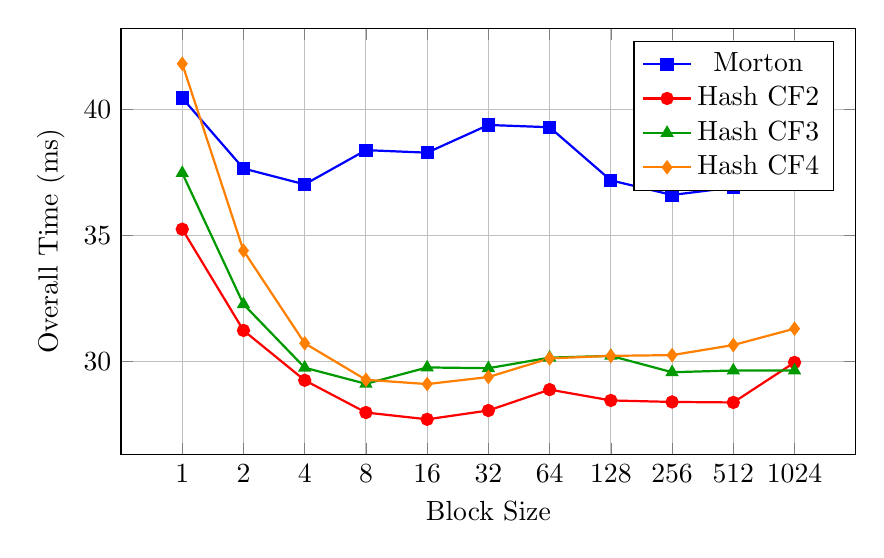
\begin{tikzpicture}
\begin{axis}[
    width=0.9\textwidth,
    height=7cm,
    xlabel={Block Size},
    ylabel={Overall Time (ms)},
    legend pos=north east,
    xmode=log,
    log basis x={2},
    xtick={1,2,4,8,16,32,64,128,256,512,1024},
    xticklabels={1,2,4,8,16,32,64,128,256,512,1024},
    grid=major,
    mark size=2pt,
]

% Morton
\addplot[color=blue,mark=square*,thick] coordinates {
    (1,40.46) (2,37.66) (4,37.03) (8,38.39) (16,38.29) 
    (32,39.39) (64,39.30) (128,37.19) (256,36.61) (512,36.91) (1024,39.67)
};

% Hash CF2
\addplot[color=red,mark=*,thick] coordinates {
    (1,35.25) (2,31.23) (4,29.25) (8,27.97) (16,27.70) 
    (32,28.05) (64,28.88) (128,28.45) (256,28.39) (512,28.37) (1024,29.96)
};

% Hash CF3
\addplot[color=green!60!black,mark=triangle*,thick] coordinates {
    (1,37.48) (2,32.27) (4,29.75) (8,29.11) (16,29.76) 
    (32,29.73) (64,30.15) (128,30.22) (256,29.57) (512,29.64) (1024,29.64)
};

% Hash CF4
\addplot[color=orange,mark=diamond*,thick] coordinates {
    (1,41.82) (2,34.40) (4,30.72) (8,29.27) (16,29.10) 
    (32,29.38) (64,30.12) (128,30.22) (256,30.25) (512,30.65) (1024,31.30)
};

\legend{Morton, Hash CF2, Hash CF3, Hash CF4}
\end{axis}
\end{tikzpicture}
\caption{Overall execution time for voxel size 0.25}
\end{figure}

% GRAPH 2: Voxel Size 0.5
\begin{figure}[H]
\centering
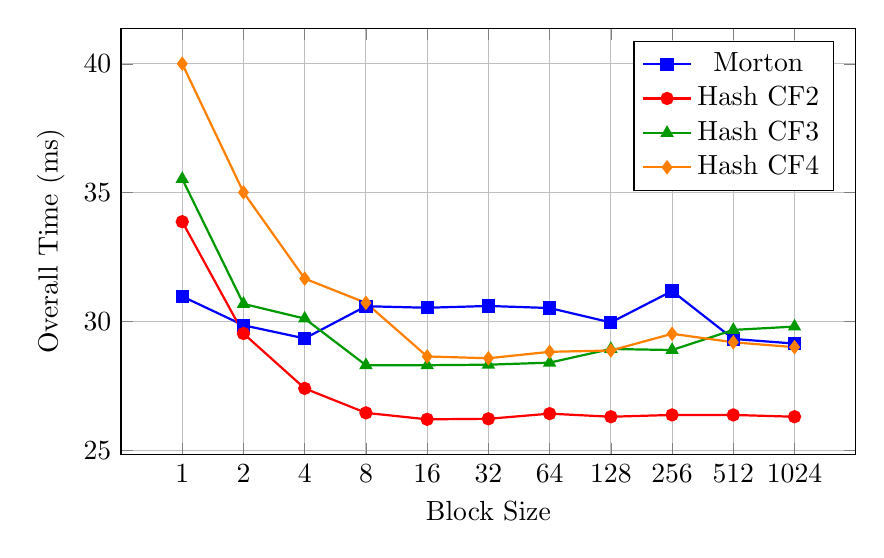
\begin{tikzpicture}
\begin{axis}[
    width=0.9\textwidth,
    height=7cm,
    xlabel={Block Size},
    ylabel={Overall Time (ms)},
    legend pos=north east,
    xmode=log,
    log basis x={2},
    xtick={1,2,4,8,16,32,64,128,256,512,1024},
    xticklabels={1,2,4,8,16,32,64,128,256,512,1024},
    grid=major,
    mark size=2pt,
]

% Morton
\addplot[color=blue,mark=square*,thick] coordinates {
    (1,30.97) (2,29.85) (4,29.34) (8,30.59) (16,30.53) 
    (32,30.60) (64,30.52) (128,29.96) (256,31.18) (512,29.32) (1024,29.14)
};

% Hash CF2
\addplot[color=red,mark=*,thick] coordinates {
    (1,33.87) (2,29.53) (4,27.40) (8,26.45) (16,26.20) 
    (32,26.22) (64,26.42) (128,26.30) (256,26.37) (512,26.37) (1024,26.30)
};

% Hash CF3
\addplot[color=green!60!black,mark=triangle*,thick] coordinates {
    (1,35.53) (2,30.68) (4,30.11) (8,28.30) (16,28.30) 
    (32,28.32) (64,28.40) (128,28.93) (256,28.89) (512,29.67) (1024,29.80)
};

% Hash CF4
\addplot[color=orange,mark=diamond*,thick] coordinates {
    (1,40.00) (2,35.01) (4,31.66) (8,30.72) (16,28.64) 
    (32,28.57) (64,28.82) (128,28.87) (256,29.52) (512,29.19) (1024,29.00)
};

\legend{Morton, Hash CF2, Hash CF3, Hash CF4}
\end{axis}
\end{tikzpicture}
\caption{Overall execution time for voxel size 0.5}
\end{figure}

% GRAPH 3: Voxel Size 0.75
\begin{figure}[H]
\centering
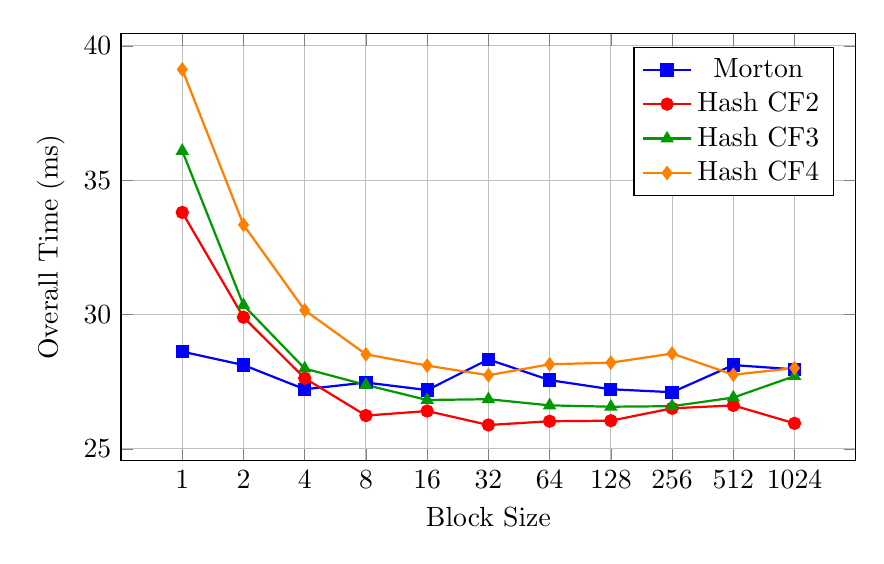
\begin{tikzpicture}
\begin{axis}[
    width=0.9\textwidth,
    height=7cm,
    xlabel={Block Size},
    ylabel={Overall Time (ms)},
    legend pos=north east,
    xmode=log,
    log basis x={2},
    xtick={1,2,4,8,16,32,64,128,256,512,1024},
    xticklabels={1,2,4,8,16,32,64,128,256,512,1024},
    grid=major,
    mark size=2pt,
]

% Morton
\addplot[color=blue,mark=square*,thick] coordinates {
    (1,28.62) (2,28.12) (4,27.22) (8,27.47) (16,27.19) 
    (32,28.33) (64,27.56) (128,27.22) (256,27.11) (512,28.12) (1024,27.96)
};

% Hash CF2
\addplot[color=red,mark=*,thick] coordinates {
    (1,33.80) (2,29.90) (4,27.63) (8,26.24) (16,26.41) 
    (32,25.89) (64,26.03) (128,26.05) (256,26.51) (512,26.62) (1024,25.95)
};

% Hash CF3
\addplot[color=green!60!black,mark=triangle*,thick] coordinates {
    (1,36.09) (2,30.35) (4,27.99) (8,27.38) (16,26.82) 
    (32,26.85) (64,26.62) (128,26.57) (256,26.59) (512,26.91) (1024,27.71)
};

% Hash CF4
\addplot[color=orange,mark=diamond*,thick] coordinates {
    (1,39.12) (2,33.34) (4,30.16) (8,28.52) (16,28.10) 
    (32,27.74) (64,28.15) (128,28.21) (256,28.55) (512,27.76) (1024,28.01)
};

\legend{Morton, Hash CF2, Hash CF3, Hash CF4}
\end{axis}
\end{tikzpicture}
\caption{Overall execution time for voxel size 0.75}
\end{figure}

% GRAPH 4: Voxel Size 1.0
\begin{figure}[H]
\centering
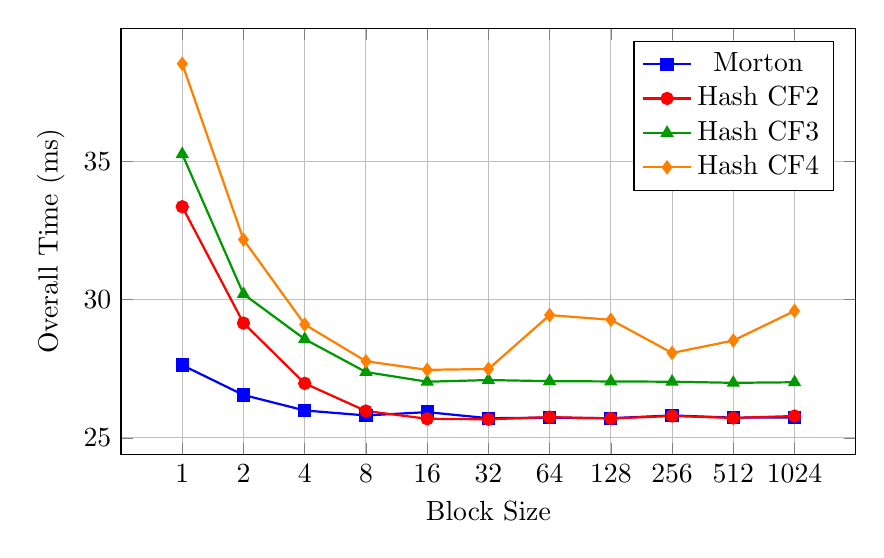
\begin{tikzpicture}
\begin{axis}[
    width=0.9\textwidth,
    height=7cm,
    xlabel={Block Size},
    ylabel={Overall Time (ms)},
    legend pos=north east,
    xmode=log,
    log basis x={2},
    xtick={1,2,4,8,16,32,64,128,256,512,1024},
    xticklabels={1,2,4,8,16,32,64,128,256,512,1024},
    grid=major,
    mark size=2pt,
]

% Morton
\addplot[color=blue,mark=square*,thick] coordinates {
    (1,27.63) (2,26.55) (4,25.99) (8,25.81) (16,25.93) 
    (32,25.71) (64,25.73) (128,25.71) (256,25.81) (512,25.73) (1024,25.74)
};

% Hash CF2
\addplot[color=red,mark=*,thick] coordinates {
    (1,33.36) (2,29.15) (4,26.97) (8,25.97) (16,25.69) 
    (32,25.67) (64,25.75) (128,25.70) (256,25.79) (512,25.72) (1024,25.79)
};

% Hash CF3
\addplot[color=green!60!black,mark=triangle*,thick] coordinates {
    (1,35.26) (2,30.20) (4,28.57) (8,27.38) (16,27.03) 
    (32,27.09) (64,27.05) (128,27.04) (256,27.03) (512,26.99) (1024,27.01)
};

% Hash CF4
\addplot[color=orange,mark=diamond*,thick] coordinates {
    (1,38.53) (2,32.17) (4,29.10) (8,27.77) (16,27.46) 
    (32,27.49) (64,29.44) (128,29.27) (256,28.07) (512,28.52) (1024,29.59)
};

\legend{Morton, Hash CF2, Hash CF3, Hash CF4}
\end{axis}
\end{tikzpicture}
\caption{Overall execution time for voxel size 1.0}
\end{figure}

% GRAPH 5: Voxel Size 1.25
\begin{figure}[H]
\centering
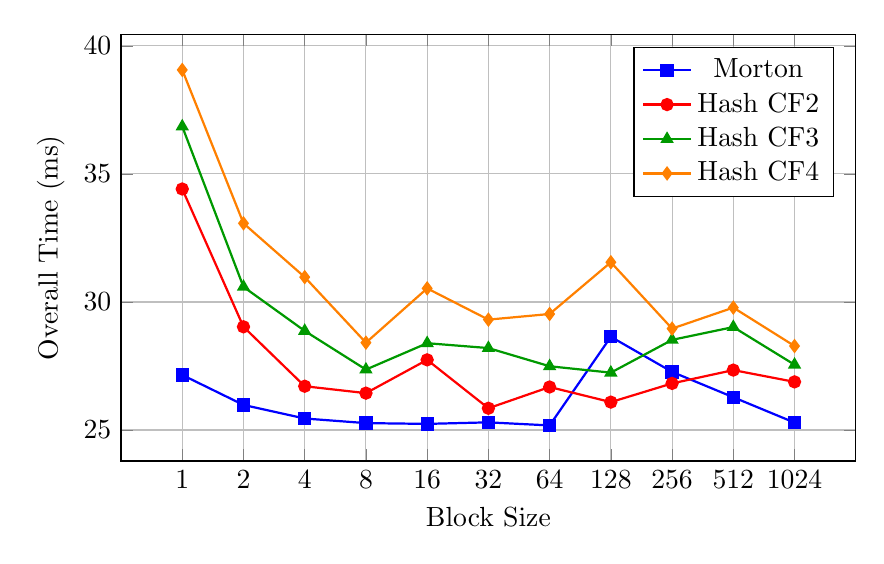
\begin{tikzpicture}
\begin{axis}[
    width=0.9\textwidth,
    height=7cm,
    xlabel={Block Size},
    ylabel={Overall Time (ms)},
    legend pos=north east,
    xmode=log,
    log basis x={2},
    xtick={1,2,4,8,16,32,64,128,256,512,1024},
    xticklabels={1,2,4,8,16,32,64,128,256,512,1024},
    grid=major,
    mark size=2pt,
]

% Morton
\addplot[color=blue,mark=square*,thick] coordinates {
    (1,27.15) (2,25.98) (4,25.45) (8,25.27) (16,25.24) 
    (32,25.30) (64,25.18) (128,28.64) (256,27.27) (512,26.28) (1024,25.29)
};

% Hash CF2
\addplot[color=red,mark=*,thick] coordinates {
    (1,34.41) (2,29.03) (4,26.71) (8,26.44) (16,27.74) 
    (32,25.85) (64,26.68) (128,26.09) (256,26.82) (512,27.34) (1024,26.88)
};

% Hash CF3
\addplot[color=green!60!black,mark=triangle*,thick] coordinates {
    (1,36.85) (2,30.59) (4,28.87) (8,27.36) (16,28.39) 
    (32,28.20) (64,27.49) (128,27.24) (256,28.52) (512,29.02) (1024,27.55)
};

% Hash CF4
\addplot[color=orange,mark=diamond*,thick] coordinates {
    (1,39.06) (2,33.07) (4,30.97) (8,28.41) (16,30.53) 
    (32,29.31) (64,29.53) (128,31.55) (256,28.96) (512,29.78) (1024,28.28)
};

\legend{Morton, Hash CF2, Hash CF3, Hash CF4}
\end{axis}
\end{tikzpicture}
\caption{Overall execution time for voxel size 1.25}
\end{figure}
\begin{thebibliography}{10}
\bibitem{Nießner2013}
M. Nießner, M. Zollhöfer, S. Izadi \& M. Stamminger, “Real-time 3D Reconstruction at Scale using Voxel Hashing,” ACM Transactions on Graphics (TOG), vol. 32, no. 6, 2013.


\bibitem{morton_forceflow}
“Morton encoding/decoding through bit interleaving: Implementations”,  
Forceflow — Jeroen Baert's Blog, 7 October 2013.  
Available online: \url{https://www.forceflow.be/2013/10/07/morton-encodingdecoding-through-bit-interleaving-implementations/}  
(Accessed: 28 November 2025).

\bibitem{thrust_cccl}
NVIDIA Corporation,  
\emph{“Thrust — CUDA Core Compute Libraries (CCCL)”}.  
Available at: \url{https://nvidia.github.io/cccl/thrust/}  
(Accessed: 28 November 2025).

\bibitem{las_file_format_wikipedia}
Wikipedia contributors,  
\emph{“LAS file format”}, Wikipedia, The Free Encyclopedia.  
Available at: \url{https://en.wikipedia.org/wiki/LAS_file_format}  
(Accessed: 28 November 2025).

\bibitem{medium_voxelization}
Ayushi Sharma,  
\emph{“From Point Clouds to Voxel Grids: A Practical Guide to 3D Data Voxelization”},  
Medium, 2021.  
Available at: \url{https://medium.com/@ayushi.sharma.3536/from-point-clouds-to-voxel-grids-a-practical-guide-to-3d-data-voxelization-cf5991c1e7bb}  
(Accessed: 28 November 2025).

\end{thebibliography}
\end{document}
